\subsection{Integrating an external image into the NanoSIMS dataset}
\setcounter{step}{0}

\goldbox{}
NanoSIMS measurements are compatible with correlative imaging. That is, it is possible to first measure a~sample with another imaging technique, such as TEM (transmission electron microscopy), SEM (scanning electron microscopy), or FM (fluorescence microscopy), and then image the very same area on the sample with NanoSIMS. To aid this type of correlative imaging, LANS implements functions that allow you to align an external image with the NanoSIMS image and then import the aligned external image into LANS for the purpose of defining ROIs, creating overlays, or conducting other quantitative analyses. This section explains how to do these steps in LANS.
\tcbe

As an example, we will use two input files: \ttt{Ecoli-Azo-Gam42a.im.zip} contains the NanoSIMS data (secondary ions of \ttt{12C}, \ttt{13C}, \ttt{19F}, \ttt{12C14N}, \ttt{32S} and \ttt{Esi}, Fig.~\ref{fig:LANS-ext-raw}A), while \ttt{Ecoli-Azo-Gam42a-FISH.tif} contains the FM data (green channel is the fluorescence intensity from a~microbe-specific FISH probe, blue channel is the fluorescence intensity of the DAPI stain attached to DNA of all microbes, Fig.~\ref{fig:LANS-ext-raw}B). These data are available from the same location as the LANS program (folder \ttt{data/Ecoli-Azo}).

\subsubsection{Aligning an external image with the NanoSIMS image}
\setcounter{step}{0}

\goldbox{}
Although the NanoSIMS and external images were obtained from the same area, it is very \emph{unlikely} that they look exactly the same: typically, they are distorted relative to each other by translation, rotation and heterogeneous stretching. Thus, in the first step, the external and NanoSIMS images need to be \bb{aligned}.
\tcbe

\s In the main LANS window, process the NanoSIMS dataset \ttt{Ecoli-Azo-Gam42a.im.zip} until you arrive at accumulated and scaled ion count images, as shown in Fig.~\ref{fig:LANS-ext-raw}A (see Section~\ref{sec:} for the relevant details).

\begin{figure}[!ht]
\centering
\begin{tabular}{cc}
A: 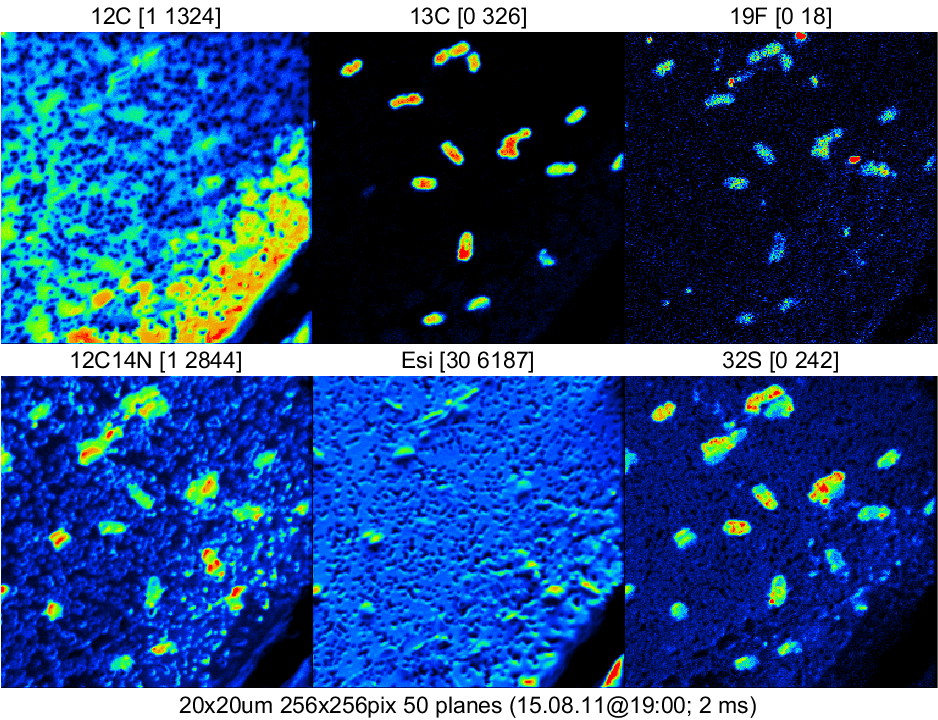
\includegraphics[scale=0.665, valign=t]{figs7/Ecoli-Azo-Gam42a}
&
\raisebox{-1.6mm}{%
\begin{tabular}[t]{cc}
B: 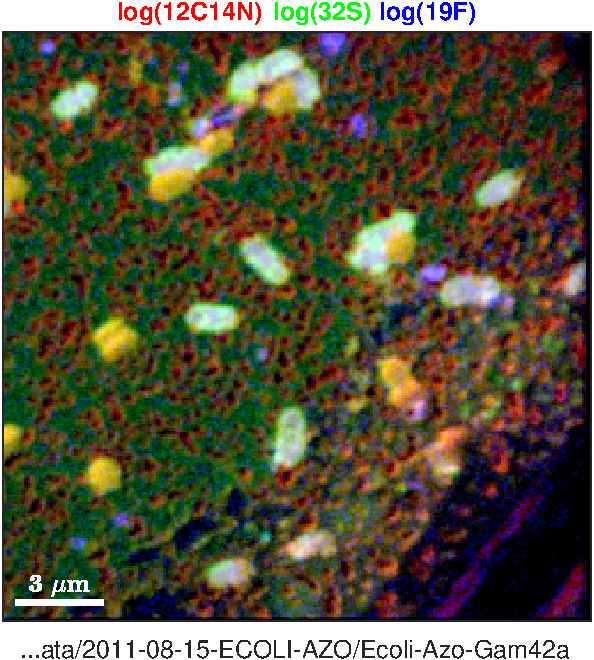
\includegraphics[scale=0.348, valign=t]{figs7/log(12C14N)-vs-log(32S)-vs-log(19F)-rgb}
\\[15mm]
C: \raisebox{-1.75mm}{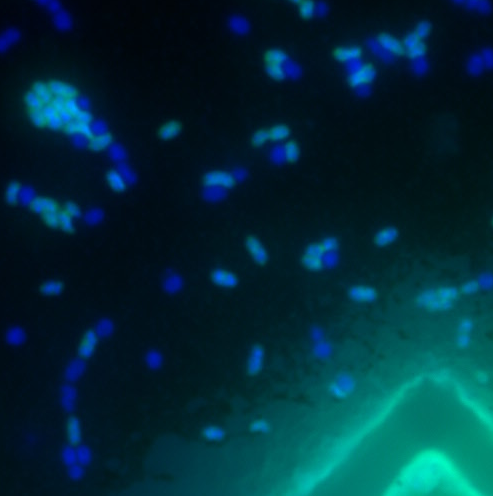
\includegraphics[scale=0.2, valign=t]{figs7/Ecoli-Azo-Gam42a-FISH}}
\end{tabular}}
\end{tabular}
\caption{\label{fig:LANS-ext-raw}%
Example of (A--B) NanoSIMS and (C) fluorescence images before their integration in LANS. Panel~A shows the accumulated images of all detected ions, panel~B shows an RGB overlay of the log-transformed counts of \ttt{12C14N}, \ttt{32S} and \ttt{19F} ions. }
\end{figure}

\s Export the ion count images or RGB overlays using \lans{Output} $\ra$ \lans{Display masses}.

\nb\bul The choice depends on what you think is the best NanoSIMS image, or an RGB overlay of NanoSIMS images, based on which you will be able to align the external image.

\bul If you plan to use one of the ion count images for aligning the external image, then the relevant image data will be exported in the Matlab format (as \ttt{*.mat} files), stored in the \ttt{mat} sub-folder.

\bul In this example, choose the RGB overlay of log-transformed counts of \ttt{12C14N} (red), \ttt{32S} (green) and \ttt{19F} (blue) ions (Fig.~\ref{fig:LANS-ext-raw}B). This overlay is exported not only in PDF but also as a~\ttt{TIF} file called \ttt{log(12C14N)-vs-log(32S)-vs-log(19F)-rgb.tif}, stored in the \ttt{tif} sub-folder.

\s Select \lans{External} $\ra$ \lans{Align external and nanosims images}.

\s In the new window that opens, select \lans{File} $\ra$ \lans{Load external image}. Navigate to the file of the external image and select it.

\nb\bul In this example, select the file \ttt{Ecoli-Azo-Gam42a-FISH.tif}, which looks as shown in Fig.~\ref{fig:LANS-ext-raw}C.

\s In the same window, select \lans{File} $\ra$ \lans{Load nanosims image}. Navigate to the file you chose in step~2.

\nb\bul In this example, select the file \ttt{log(12C14N)-vs-log(32S)-vs-log(19F)-rgb.tif}.

\s Select \lans{Action} $\ra$ \lans{Add point} (\ttt{Ctrl+a}), then click within the \bb{external} image (\bb{left} panel) on a~point for which you will be able to find a~corresponding point in the NanoSIMS image (right panel).

\nb\bul After you select a point, you can use arrow keys to fine-tune its position. Press \ttt{Enter} when you are certain with the position.

\s Again, select \lans{Action} $\ra$ \lans{Add point} (\ttt{Ctrl+a}), but this time click within the \bb{NanoSIMS} image (\bb{right} panel) on a~point that correponds to the point on the external image defined in the previous step. 

\nb\bul Again, use arrow keys to fine-tune the point's position and press \ttt{Enter} to confirm it.

\s Repeat steps 6 and 7 several times to define additional points in the external image and the corresponding points in the NanoSIMS image, one pair of points at a~time.

\nb\bul The more point pairs you define, the better the alignment will be. You will need at least 4~point pairs for a~reasonably good alignment. 

\bul An example of point pairs defined in this example is shown in Fig.~\ref{fig:LANS-ext-window}.

\begin{figure}[!ht]
\centering
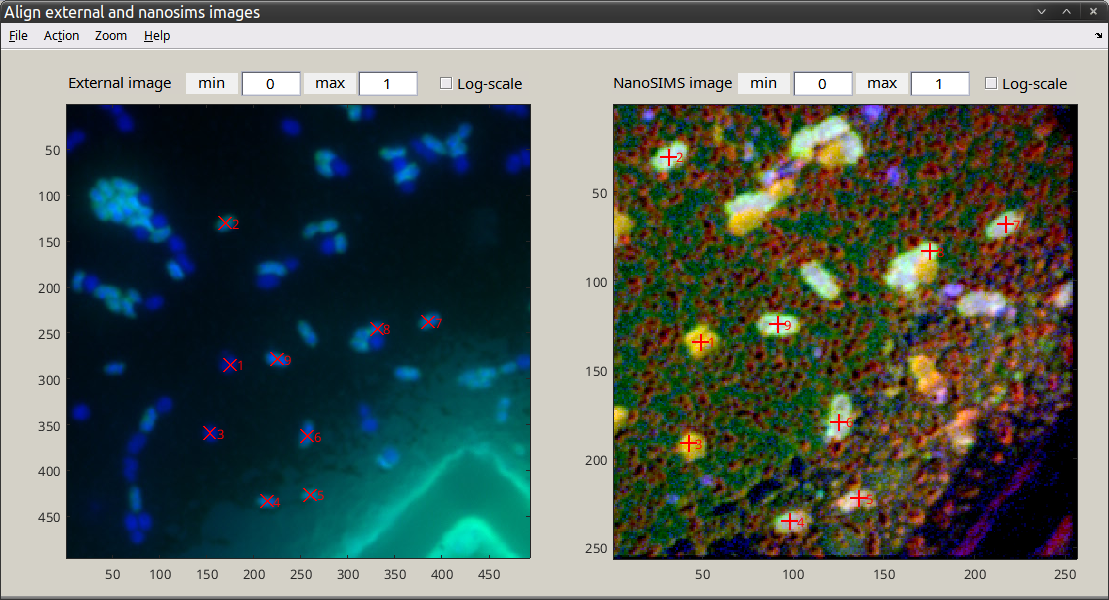
\includegraphics[width=0.9\textwidth]{figs7/LANS-ext-align-points}
\caption{\label{fig:LANS-ext-window}%
Example of point pairs defined in the external (left panel) and NanoSIMS (right panel) images. Points with the same identification number correspond to each other. These points are defined manually by the user based on distinct features in the images, such as cells in this example.}
\end{figure}

\bul Note that each added point will have a~unique identification number. You will be able to see which points correspond to each other in the external and NanoSIMS images based on these identification numbers.

\bul If you need to change the color of the point or an identifier, you can do this by selecting \lans{Action} $\ra$ \lans{Change point's color}.

\s If you need to modify a~point's location, select \lans{Action} $\ra$ \lans{Modify point}, then click on the point you want to modify and press \ttt{Enter} to confirm the selection. Subsequently, use arrow keys to modify the point's location, and finally press \ttt{Enter} to confirm thew new location.

\nb\bul Observe messages in the Matlab console for more details about what exactly you need to do.

\s If you need to remove a~pair of corresponding points, select \lans{Action} $\ra$ \lans{Remove pair of points}, then click on one of the points in the pair and press \ttt{Enter} to confirm the removal.

 \s After defining a reasonably high number of point pairs (typically 5--10 should be sufficient), select \lans{File} $\ra$ \lans{Save point list} to save the points' coordinates in a~matlab file. 
 
 \nb\bul You can load these coordinates later via \lans{File} $\ra$ \lans{Load point list}. Subsequently, you can add more points, modify points, or remove points, as described in steps 6--10.

\s If the selected NanoSIMS image does not contain all features based on which you can align the external image, you can load a~\bb{different} NanoSIMS image at any time (see step~5). When doing so, you may need to select \lans{Action} $\ra$ \lans{Update points} to redraw the currently defined points in the image.

\s Select \lans{Action} $\ra$ \lans{Alignment based on N$>$4 points} to \bb{perform the image alignment} based on the defined point pairs.

\nb\bul
The result will be displayed in a~new window (Fig.~\ref{fig:LANS-ext-result}). You can quality-check the alignment by changing the transparency of the layers displaying the external and NanoSIMS images through the \lans{Transparency} menu or, more quickly, by pressing \ttt{Ctrl+1} -- \ttt{Ctrl+4} keys.

\begin{figure}[!ht]
\centering
\begin{tabular}{ccc}
A & B & C \\
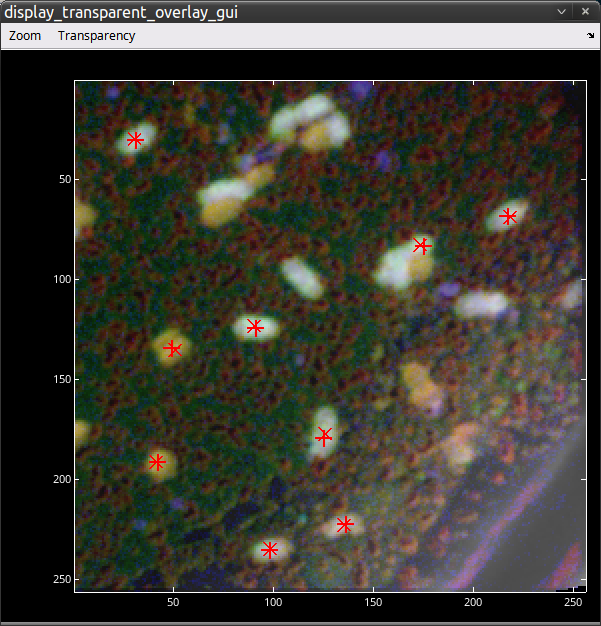
\includegraphics[scale=0.23]{figs7/LANS-ext-result1}
&
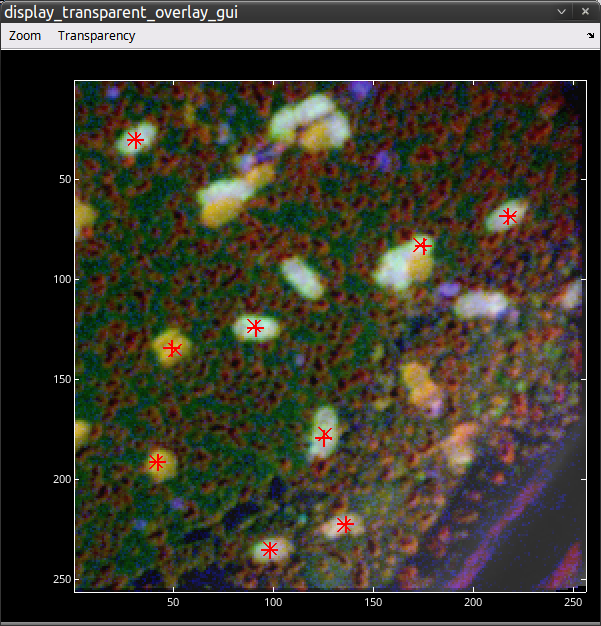
\includegraphics[scale=0.23]{figs7/LANS-ext-result2}
&
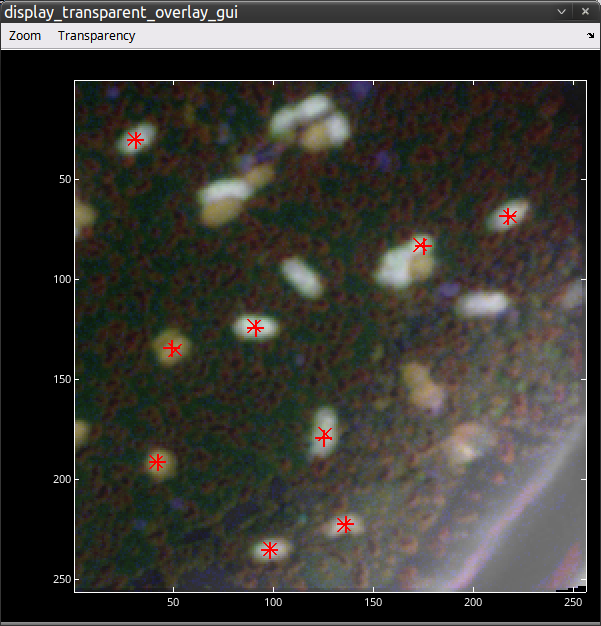
\includegraphics[scale=0.23]{figs7/LANS-ext-result3}
\end{tabular}
\caption{\label{fig:LANS-ext-result}%
Results of the image alignment are shown as an overlay. Panels (A--C) show the overlays at different levels of transparency of the external and nanoSIMS image layers. These levels can be changed through the \lans{Transparency} menu. Note the match between the point pairs defined in the external ($\times$) and nanoSIMS ($+$) images. Although the external image was originally an RGB image in this example, the image is converted to a~grayscale in the overlay.}
\end{figure}

\s If you are satisfied with the result, select \lans{Action} $\ra$ \lans{Export aligned external image} to \bb{store the aligned external image} for later use. If not, repeat steps~6--13.

\nb\bul Specify an appropriate name (e.g., \ttt{ext\_aligned}) and location of the file. You can store it in a~Matlab (\ttt{*.mat}) or TIF (\ttt{*.tif}) format. It is a~good idea to store them in both formats and in the folder with all the other processed data.

%%%

\subsubsection{Importing an aligned external image}
\setcounter{step}{0}

\goldbox{}
Once the external image is aligned with the NanoSIMS images, it can be imported into LANS using the following steps.
\tcbe

\s In the main LANS window, select \lans{External} $\ra$ \lans{Select aligned external image}, navigate to the image, and click \lans{Open} to select it. 

\nb\bul If the external image is an~RGB image, as in this example, you will be asked to select \bb{one} channel (\ttt{r}, \ttt{g}, or \ttt{b}) to fully define the external image. This is because currently LANS only supports a~single-channel (i.e., grascale) external images. In this example, choose channel \lanstf{g} to load the channel corresponding to the fluorescence from the microbe-specific FISH probe.

\s Read carefully the note that appears after you load the image. It tells you that the external image has been \bb{integrated} into the NanoSIMS dataset and can be used as a~\bb{regular mass} with the name \lanstf{ext}.

%%%%

\subsubsection{Using the external image with the NanoSIMS images}
\setcounter{step}{0}

\goldbox{}
After importing the aligned external image into LANS, the image can be used, effectively, as if it were one of the masses in the NanoSIMS dataset. By default, the name of this `extra mass' is \lanstf{ext}. This name can then be used, for instance, as a~template for ROI definition or to create overlays with NanoSIMS images or scatter plots, as described in the following example.
\tcbe

\s Type \ttt{ext} into one of the ratio \lanstf{expression} text fields, specify the \lanstf{scale} (e.g., you can start with \ttt{[0 1]}), and press \ttt{Enter} to display the scaled external image.

\nb\bul This will reassure you that the external image is really usable as part of the NanoSIMS dataset.

\s To use the external image for defining ROIs, type \ttt{ext} in the \lanstf{ROI definition template} and proceed as described in Section~\ref{sec:} to define ROIs.

\nb\bul This is an example where \lans{Interactive thresholding} will really speed up the  ROI definition.

\bul After using the green channel of the external image as a~template, the ROIs may look as shown in Fig.~\ref{fig:LANS-ext-ROIs}A.

\def\scf{0.22}
\begin{figure}[!ht]
\centering
\begin{tabular}{ccc}
A & B & C \\
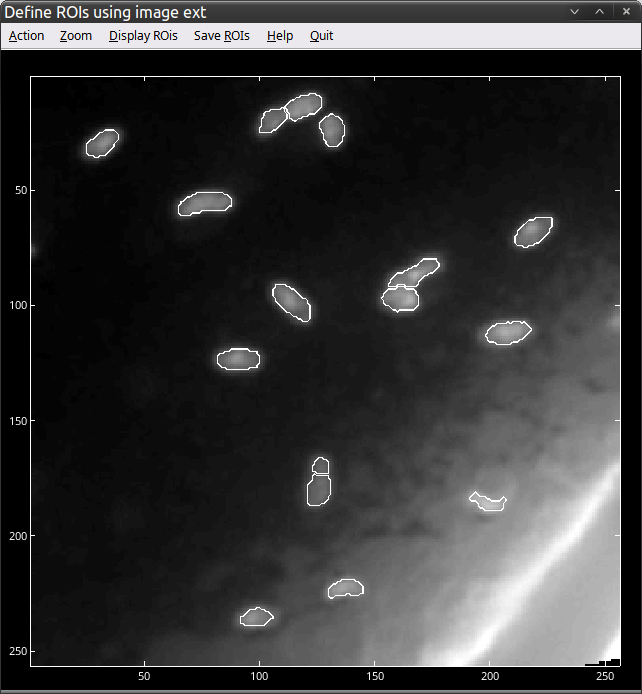
\includegraphics[scale=\scf]{figs7/LANS-ext-ROIs1}
&
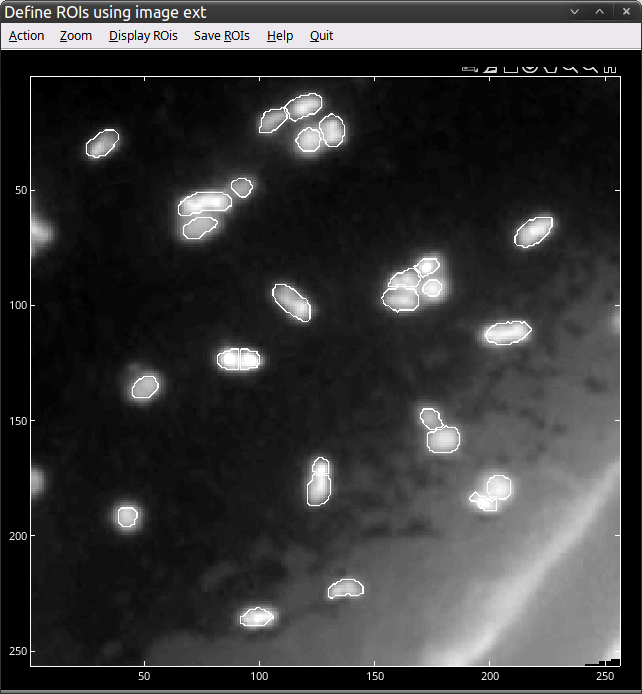
\includegraphics[scale=\scf]{figs7/LANS-ext-ROIs2}
&
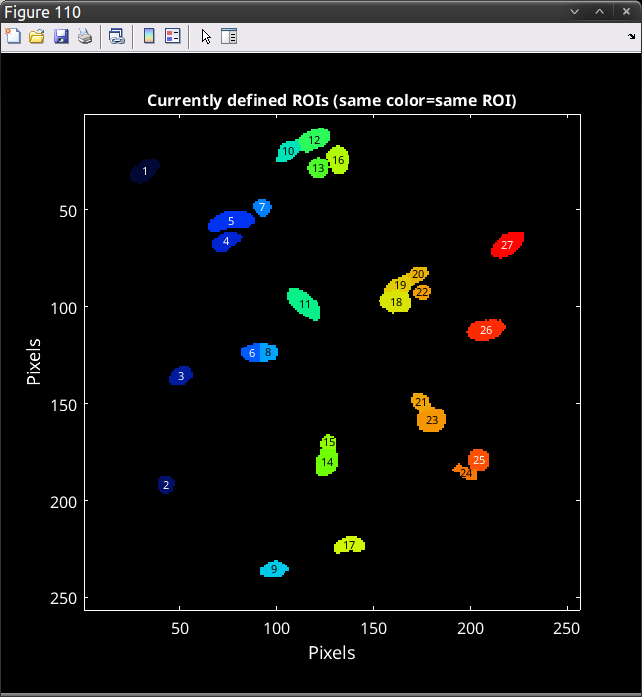
\includegraphics[scale=\scf]{figs7/LANS-ext-ROIs3}
\end{tabular}
\caption{\label{fig:LANS-ext-ROIs}%
ROI definition using an aligned external image. (A) First set of ROIs defined based on the green channel of the external image. (B) Added and revised ROIs defined based on the blue channel of the external image. (C) Final set of ROIs.}
\end{figure}

\goldbox{}
This step is specific to this particular example, but it gives you an idea about the \emph{iterative} process of using an external image during NanoSIMS data processing. 
\tcbe

\s Based on the original external image, it is clear that not all cells are visible in the green channel. To define all cells in the image, the blue channel needs to be used instead. Thus, import the external image again as described in the previous section, but this time choose channel \lanstf{b} (DAPI flurescence) instead of \lanstf{g}. Then proceed with step~2 to continue ROI definition.

\nb\bul After using the blue channel of the external image as a~template, the revised ROIs may look as shown in Fig.~\ref{fig:LANS-ext-ROIs}B.

\s Classify the ROIs using steps described in Section~\ref{sec:}.

\nb\bul
You can base this classification on the aligned external image, where you clearly see (in most cases) the differences between cells only stained with DAPI (blue) and cells stained with both DAPI and the FISH probe (cyan). You can use, for instance, \ttt{b} and \ttt{c} as the class names for the respective cells.

\s Type \ttt{ext/pixel} into one of the ratio \lanstf{expression} text fields and specify the \lanstf{scale}.

\nb\bul This is necessary if you want to properly normalize the ROI-specific values for the external image data.

\s Create overlays between the external image and one of the NanoSIMS images, or scatter plots between the ROI-specific values in the external and NanoSIMS images, using steps described in Section~\ref{sec:}. 

\nb\bul Examples of the results may look as shown in Fig.~\ref{fig:LANS-ext-overlays}.

\def\scf{0.42}
\begin{figure}[!ht]
\centering
\begin{tabular}{cc}
A: 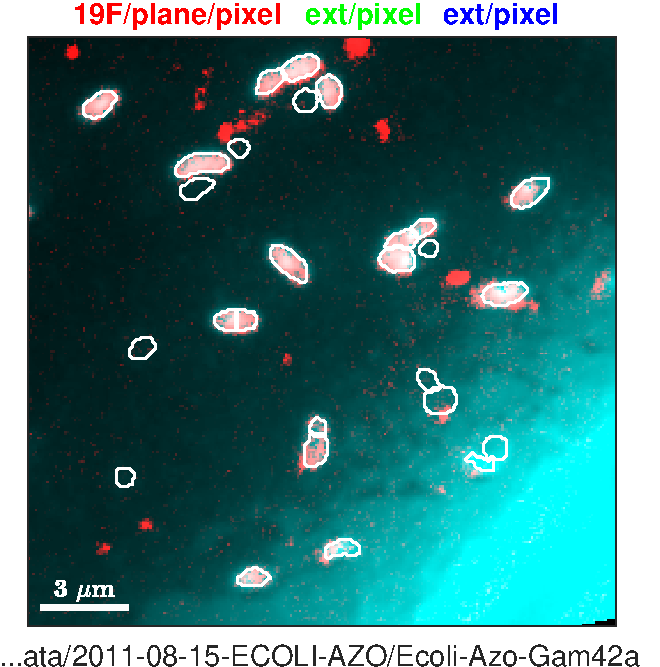
\includegraphics[scale=\scf, valign=t]{figs7/19F-plane-pixel-vs-ext-pixel-vs-ext-pixel-rgb}
&
B: 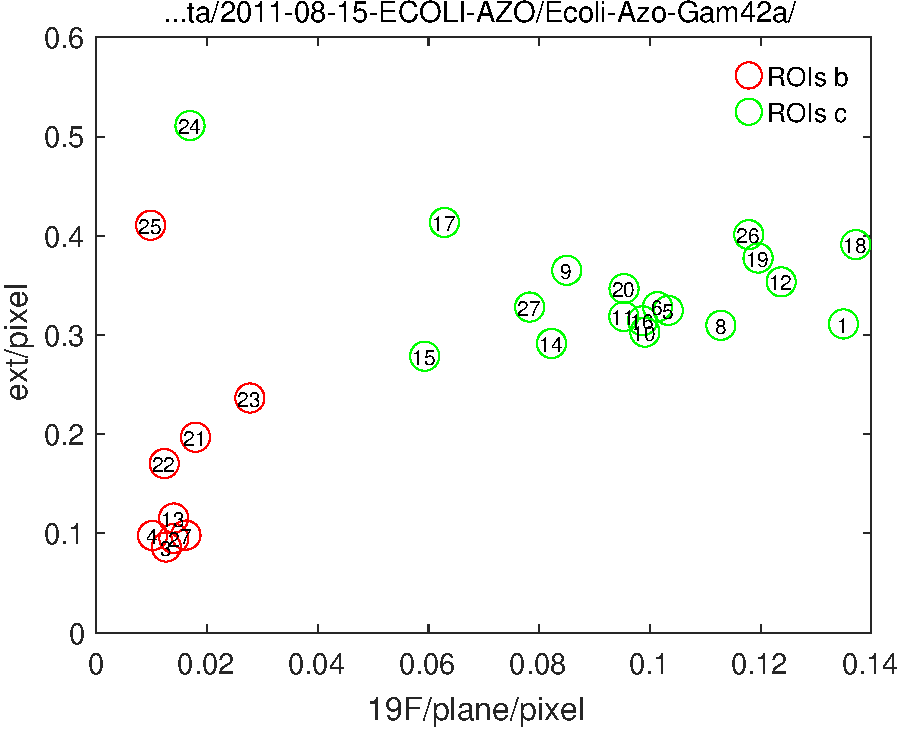
\includegraphics[scale=\scf, valign=t]{figs7/19F-plane-pixel-vs-ext-pixel}
\\
{ } & { } \\
C: 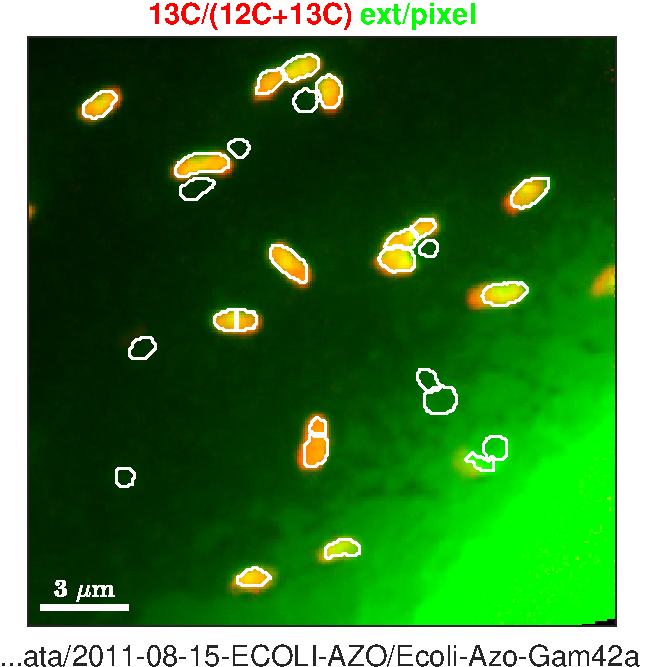
\includegraphics[scale=\scf, valign=t]{figs7/13C-(12C+13C)-vs-ext-pixel-rgb}
&
D: 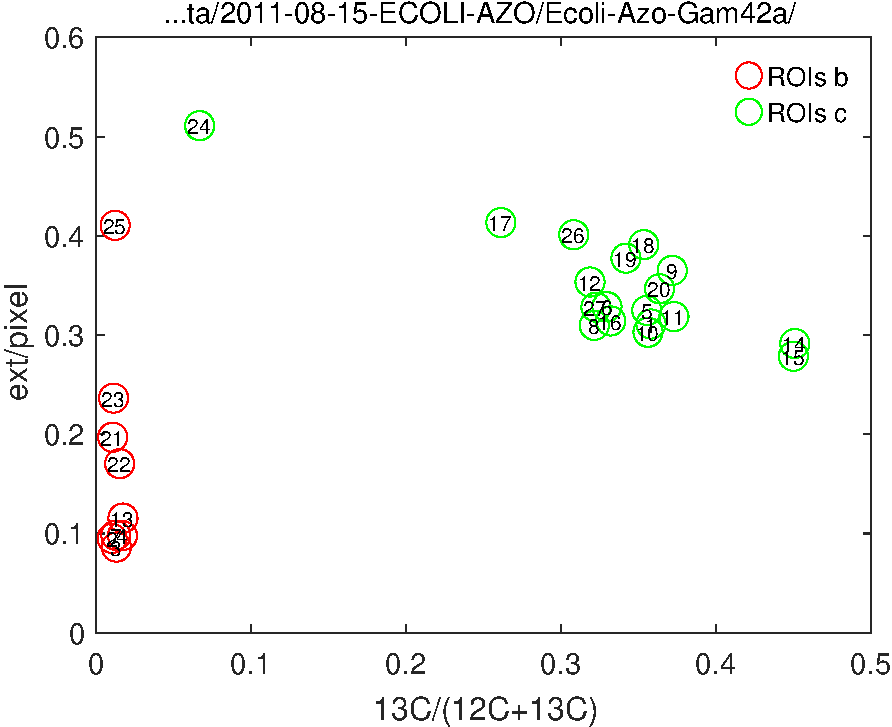
\includegraphics[scale=\scf, valign=t]{figs7/13C-(12C+13C)-vs-ext-pixel}
\end{tabular}
\caption{\label{fig:LANS-ext-overlays}%
Examples of results combining ROI-specific values derived from the external and NanoSIMS images. They show that in most cells, there is a~clear correspondence between the ROI-specific intensity of the \ttt{19F} ion counts and the FISH signal (panels A--B). They also show that most of the FISH-stained cells are highly enriched in the ${}^{13}C$ isotope and vice versa (C--D). Cells for which these statements are not valid require closer inspection.}
\end{figure}

\s When you are finished using the external image, it is a~good idea to \bb{remove} it from the NanoSIMS dataset. You can do this by selecting \lans{External} $\ra$ \lans{Select aligned external image} and clicking \lans{Cancel}. Also, do not forget to store preferences at the end of your analysis.

%%%%

\subsubsection{Resampling of NanoSIMS images to match resolution of an external image}
\setcounter{step}{0}

\goldbox{}
In addition to rotation, stretching or other types of image distortion, it can happen that the external and NanoSIMS images have a~very different pixel resolution. For example, in the example below, the TEM image has roughly 10-fold higher resolution than the NanoSIMS image. If you want to use such a~high-resolution TEM image as a~template for defining ROIs, which can then be used to quantify ROI-specific NanoSIMS data such as ion counts or ratios, it is necessary to rescale the NanoSIMS images to match the resolution of the external image. This can be done by resampling the NanoSIMS images, as described in the following steps.
\tcbe

\nb Work in progress.

